\documentclass[8pt]{extarticle}
\title{}
\author{Avinash Iyer}
\date{}
\usepackage[shortlabels]{enumitem}

%font setup
%
%\usepackage[math]{anttor}

%paper setup
\usepackage{geometry}
\geometry{letterpaper, portrait, margin=1in}
\usepackage{fancyhdr}

%symbols
\usepackage{amsmath}
\usepackage{mathtools}
\usepackage{amssymb}
\usepackage{hyperref}
\usepackage{gensymb}

\usepackage[T1]{fontenc}
\usepackage[utf8]{inputenc}

%chemistry stuff
\usepackage[version=4]{mhchem}
\usepackage{chemfig}

%plotting
\usepackage{pgfplots}
\usepackage{tikz}

%\usepackage{natbib}

%graphics stuff
\usepackage{graphicx}
\graphicspath{ {./images/} }

%code stuff
%when using minted, make sure to add the -shell-escape flag
%you can use lstlisting if you don't want to use minted
%\usepackage{minted}
%\usemintedstyle{pastie}
%\newminted[javacode]{java}{frame=lines,framesep=2mm,linenos=true,fontsize=\footnotesize,tabsize=3,autogobble,}
%\newminted[cppcode]{cpp}{frame=lines,framesep=2mm,linenos=true,fontsize=\footnotesize,tabsize=3,autogobble,}

\usepackage{listings}
\usepackage{color}
\definecolor{dkgreen}{rgb}{0,0.6,0}
\definecolor{gray}{rgb}{0.5,0.5,0.5}
\definecolor{mauve}{rgb}{0.58,0,0.82}

\lstset{frame=tb,
	language=Java,
	aboveskip=3mm,
	belowskip=3mm,
	showstringspaces=false,
	columns=flexible,
	basicstyle={\small\ttfamily},
	numbers=none,
	numberstyle=\tiny\color{gray},
	keywordstyle=\color{blue},
	commentstyle=\color{dkgreen},
	stringstyle=\color{mauve},
	breaklines=true,
	breakatwhitespace=true,
	tabsize=3
}
% text + color boxes
\usepackage{tcolorbox}
\tcbuselibrary{breakable}
\newtcolorbox{problem}[1]{colback = white, title = {#1}, breakable}
\newtcolorbox{solution}{colback = white, colframe = black!75!white, title = Solution, breakable}
%including PDFs
\usepackage{pdfpages}
\setlength{\parindent}{0pt}

\pagestyle{fancy}
\fancyhf{}
\rhead{Avinash Iyer}
\lhead{Homework Section 1.3, Individual}
\begin{document}
  \begin{problem}{1.3.3}
    Let $u$ and $v$ be adjacent vertices in $G$. Prove that $uv$ belongs to at least $d(u) + d(v) - n(G)$ triangles in $G$.
  \end{problem}
  \begin{problem}{1.3.4}
    Prove that the graph below is isomorphic to $Q_4$.
    \begin{center}
      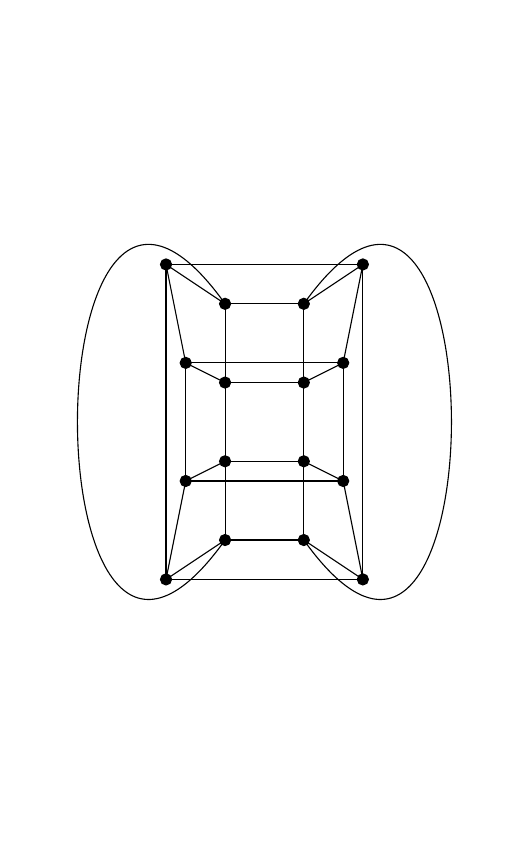
\begin{tikzpicture}
        % \draw[thin, gray] (-3,-3) grid (3,3);
        % drawing points
        \filldraw (0.5,0.5) circle (2pt);
        \filldraw (-0.5,0.5) circle (2pt);
        \filldraw (0.5,-0.5) circle (2pt);
        \filldraw (-0.5,-0.5) circle (2pt);
        \filldraw (1,0.75) circle (2pt);
        \filldraw (-1,0.75) circle (2pt);
        \filldraw (-1,-0.75) circle (2pt);
        \filldraw (1,-0.75) circle (2pt);
        \filldraw (0.5,1.5) circle (2pt);
        \filldraw (-0.5,1.5) circle (2pt);
        \filldraw (-0.5,-1.5) circle (2pt);
        \filldraw (0.5,-1.5) circle (2pt);
        \filldraw (1.25,2) circle (2pt);
        \filldraw (-1.25,2) circle (2pt);
        \filldraw (1.25,-2) circle (2pt);
        \filldraw (-1.25,-2) circle (2pt);
        % drawing lines
        \draw (0.5,0.5) -- (-0.5,0.5) -- (-0.5,-0.5) -- (0.5,-0.5) -- (0.5,0.5);
        \draw (-1.25,-2) -- (1.25,-2) -- (1.25,2) -- (-1.25,2) -- (-1.25,-2);
        \draw (1,0.75) -- (-1,0.75) -- (-1,-0.75) -- (1,-0.75) -- (1,0.75);
        \draw (0.5,1.5) -- (0.5,0.5);
        \draw (-0.5,1.5) -- (-0.5,0.5);
        \draw (-0.5,-1.5) -- (-0.5,-0.5);
        \draw (0.5,-1.5) -- (0.5,-0.5);
        \draw (0.5,-1.5) -- (-0.5,-1.5);
        \draw (0.5,1.5) -- (-0.5,1.5);
        \draw (1.25,2) -- (0.5,1.5);
        \draw (-1.25,2) -- (-0.5,1.5);
        \draw (-1.25,-2) -- (-0.5,-1.5);
        \draw (1.25,-2) -- (0.5,-1.5);
        \draw (1,0.75) -- (1.25,2);
        \draw (-1,0.75) -- (-1.25,2);
        \draw (-1,-0.75) -- (-1.25,-2);
        \draw (1,-0.75) -- (1.25,-2);
        \draw (1,0.75) -- (0.5,0.5);
        \draw (1,-0.75) -- (0.5,-0.5);
        \draw (-1,-0.75) -- (-0.5,-0.5);
        \draw (-1,0.75) -- (-0.5,0.5);
        \draw (0.5,1.5) .. controls (3,5) and (3,-5) .. (0.5,-1.5);
        \draw (-0.5,1.5) .. controls (-3,5) and (-3,-5) .. (-0.5,-1.5);
      \end{tikzpicture} 
    \end{center}
  \end{problem}
  \begin{problem}{1.3.6}
    Given graphs $G$ and $H$, determine the number of components and maximum degree in $G+H$ in terms of the parameters for $G$ and $H$.
  \end{problem}
  \begin{problem}{1.3.7}
    Determine the maximum number of edges in a bipartite subgraph of $P_n$, $C_n$, and $K_n$.
  \end{problem}
  \begin{problem}{1.3.26 (a)}
    Count the $6$-cycles in $Q_3$.
  \end{problem}
\end{document}
